\documentclass[a4paper,12pt]{article} % добавить leqno в [] для нумерации слева

%%% Содержание
\usepackage{hyperref}
\hypersetup{
    colorlinks,
    citecolor=black,
    filecolor=black,
    linkcolor=black,
    urlcolor=black
}
%%% Графика
\usepackage{graphicx}
%%% Код программы
\usepackage{listings}
%%% Работа с русским языком
\usepackage{cmap}                   % поиск в PDF
\usepackage{mathtext}               % русские буквы в формулах
\usepackage[T2A]{fontenc}           % кодировка
\usepackage[utf8]{inputenc}         % кодировка исходного текста
\usepackage[english,russian]{babel} % локализация и переносы

%%% Дополнительная работа с математикой
\usepackage{amsmath,amsfonts,amssymb,amsthm,mathtools} % AMS
\usepackage{icomma} % "Умная" запятая: $0,2$ --- число, $0, 2$ --- перечисление

%% Номера формул
\mathtoolsset{showonlyrefs=true} % Показывать номера только у тех формул, на которые есть \eqref{} в тексте.

%% Шрифты
\usepackage{euscript}    % Шрифт Евклид
\usepackage{mathrsfs} % Красивый матшрифт

%% Свои команды
\DeclareMathOperator{\sgn}{\mathop{sgn}}

%% Перенос знаков в формулах (по Львовскому)
\newcommand*{\hm}[1]{#1\nobreak\discretionary{}
    {\hbox{$\mathsurround=0pt #1$}}{}}

\lstset{language=C++}
\begin{document} % конец преамбулы, начало документа
    \begin{titlepage}
        \centering
        {\scshape\LARGE Национальный исследовательский 
            университет «Высшая школа экономики \par}
        \vspace{1cm}
        {\scshape\Large Домашняя работа по дисциплине:
            Алгоритмы и структуры данных\par}
        \vspace{1.5cm}
        {\huge\bfseries Контрольное домашнее задание\par}
        \vspace{2cm}
        \raggedleft
        {\Large Выполнил:
            \\Суровцев М.А.
            \\группа БПИ151
            \vspace{0.5cm}
            \\Преподаватель: 
            \\Мицюк А.А.\par}
        \vfill
        \centering
        {\large \today\par}
    \end{titlepage}
    \tableofcontents
    \newpage
    
    \section{Постановка задачи}
    \begin{enumerate}
        \item
        Реализовать с использованием языка C++ программы для архивирования и
        разархивирования текстовых файлов. При этом использовать два известных 
        алгоритма кодирования информации:
        \begin{itemize}
            \item
            Хаффмана (простой),
            \item
            Шеннона-Фано.
        \end{itemize}
        \item
        Провести вычислительный эксперимент с целью оценки реализованных
        алгоритмов архивации / разархивации. Оценить количество элементарных операций
        каждого алгоритма.
        \item 
        Подготовить отчет по итогам работы, содержащий постановку задачи, описание
        алгоритмов и задействованных структур данных, описание реализации, обобщенные
        результаты измерения эффективности алгоритмов, описание использованных
        инструментов (например, если использовались скрипты автоматизации), выводы о
        соответствии результатов экспериментальной проверки с теоретическими оценками
        эффективности исследуемых алгоритмов.
    \end{enumerate}
    \newpage
    
    \section{Описание алгоритмов и использованных\\ структур данных}
    \subsection{Алгориим архивирования}
    Оба алгоритма работают следующим образом (функция Compress):
    \begin{enumerate}
        \item
        Посимвольное считывание из текстового файла и построение таблицы частот
        встречаемости символов (функция BuildFrequencyTable)
        \item
        Построение бинарного кодового дерева (указатель на функцию BuildTree)
        \item
        Построение префиксных кодов путем рекурсивного обхода дерева (функция GetCharCodes)
        \item
        Запись в бинарный файл (функция CreateCompressedFile):
    \end{enumerate}
    \subsection{Алгориим разархивирования}
    Оба алгоритма работают следующим образом (функция Decompress):
    \begin{enumerate}
        \item
        Считывание таблицы частот из бинарного файла (функция BuildFrequencyTable)
        \item
        Построение бинарного кодового дерева (указатель на функцию BuildTree)
        \item
        Считывание кодов символов из бинарного файла, их декодирование путем
        рекурсивного обхода дерева (функция TranslateCodes)
    \end{enumerate}
    Единственное различие алгоритмов --- построение кодового дерева. Для этого в объявлении функции Compress/Decompress используется указатель на функцию BuildTree. 
    В зависимости от выбранного способа архивирования/разархивирования, в функцию Compress/Decompress передается 
    BuildHuffmanTree или BuildSFTree.
    \subsection{Описание основных функций}
    \begin{itemize}
        \item
        BuildFrequencyTable:
        \begin{itemize}
            \item 
            Если выполняется архивирование, то
            \begin{enumerate}
                \item
                Посимвольное считывание из текстового файла,
                \item
                Если очередной символ уже встречался, частота его появления инкреметируется, иначе символ 
                добавляется в таблицу со значением 0. (см. frequency\char`_table, п. 2.4) 
            \end{enumerate}
            \item 
            Если выполняется разархивирование, то
            \begin{enumerate}
                \item
                Считывание размера таблицы (n),
                \item
                В цикле от 0 до n - 1 считывается символ, его частота,
                \item
                Полученные данные записываются в таблицу. (см. frequency\char`_table, п. 2.4)                
            \end{enumerate}
        \end{itemize}
        \item BuildHuffmanTree
        \begin{enumerate}
            \item
            На основании таблицы частот создаются вершины (см. struct Node, п. 2.4) и записываются в очередь с 
            приоритетами (см. priority\char`_queue<Node *, vector<Node *>, CountCompare> nodes, п. 2.4), в которой 
            элементы сраниваются по убыванию частоты встречаемости,
            \item
            До тех пор, пока не останется ровно одна вершина, из очереди извлекаются две вершины и строится новая 
            вершина, указатели left и right которой ссылаются на извлеченные вершины, 
            \item
            Новая вершина добавляется в очередь.
        \end{enumerate}
        \item BuildSFTree
        \begin{enumerate}
        \item
        На основании таблицы частот создаются вершины (см. Node, 
        п. 2.4) и записываются в вектор (см. vector <Node *> 
        nodes, п. 2.4),
        \item
        Вектор сортируется по убыванию частоты встречаемости,
        \item
        Вызывается функция Divide от вектора (см. далее).
        \end{enumerate}
        \item Divide
        \begin{enumerate}
            \item
            Если в векторе осталась одна вершина, то она является листом в кодом дереве,
            \item
            Вектор делится на две части, суммы частот которых примерно равны,
            \item
            Функция Divide рекурсивно вызывается от левой и правой  частей вектора.
        \end{enumerate}
        \item CreateCompressedFile
        \begin{enumerate}
        \item
        Запись размера таблицы частот,
        \item
        Запись самой таблицы частот,
        \item
        Посимвольное считывание из текстового файла, запись кодов символов
        в бинарный файл.
        \end{enumerate}
        \item GetCharCodes
        \begin{enumerate}
            \item
            Если левый потомок вершины непустой, добавляем к коду 0,
            рекурсивно вызываем функцию от этой вершины,
            \item
            Если правый потомок вершины непустой, добавляем к коду 1,
            рекурсивно вызываем функцию от этой вершины,
            \item
            Как только в вершине оказался непустой символ, записываем его код в таблицу (см. map<char, vector<int> > 
            codes, п. 2.4) и возвращаемся на одну вершину вверх.
        \end{enumerate}
        \item TranslateCodes
        \begin{enumerate}
            \item
            Чтение размера таблицы частот,
            \item
            Чтение самой таблицы частот,
            \item
            Построение дерева на основании таблицы частот,
            \item
            Побайтовое считывание из файла до его конца,
            \item
            Если конкретный бит равен 1, то идем к правому потомку дерева,
            если конкретный бит равен 0, то идем к левому потомку.
            \item
            Как только в вершине оказался непустой символ, записываем его в текстовый файл.
        \end{enumerate}
    \end{itemize}
    \newpage
    \subsection{Структуры данных}
    Для хранения и обработки промежуточных значений были использованы следующие
    структуры данных:
    \begin{lstlisting}
        // Code tree node
        struct Node
        {
            char value = '\0';
            int frequency = 0;
            Node *left = nullptr;
            Node *right = nullptr;
        };
        // Frequency table
        map<char, unsigned> frequency_table
        // Huffman or Shannon-Fano codes
        map<char, vector<int> > codes 
        // Temporary container for nodes (Huffman)
        priority_queue<Node *, vector<Node *>, CountCompare> nodes
        // Temporary container for nodes (Shannon-Fano)
        vector<Node *> nodes
    \end{lstlisting}
    \newpage
    
    \section{Описание плана эксперимента}
    \begin{enumerate}
        \item 
        Подготовить тестовый набор из нескольких текстовых файлов разного объема
        (20, 40, 60, 80, 100 Кб; 1, 2, 3 Мб — всего 8 файлов) на разных языках (ru, en -
        кодировка UTF-8) с разным набором символов в каждом файле.
        \item
        Измерить (экспериментально) количество операций (в рамках модели
        RAM), выполняемых за время работы (архивирования,
        разархивирования) каждого алгоритма на нескольких различных
        (не менее трех) файлах для каждого размера входного файла
        и набора символов (итого получается 8 * 3 * 3 = 72 эксперимента
        по архивированию и 72 по разархивированию для каждого алгоритма,
        т. е. всего минимум 144 * 2 = 288).
        \item
        Результаты эксперимента представить в виде графиков и таблиц, сформулировать выводы.
    \end{enumerate}
    \newpage
    \section{Результаты экспериментов}
    %%%--------------------------------------------1
    \begin{figure}[!htb]
        \caption{Алгоритм Хаффмана, архивирование малых файлов}
        \centering
        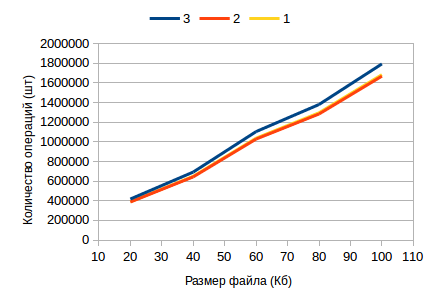
\includegraphics[width=0.5\textwidth]{graphs/1/hc_kb}
    \end{figure}
    \begin{figure}[!htb]
        \caption{Алгоритм Хаффмана, архивирование больших файлов}
        \centering
        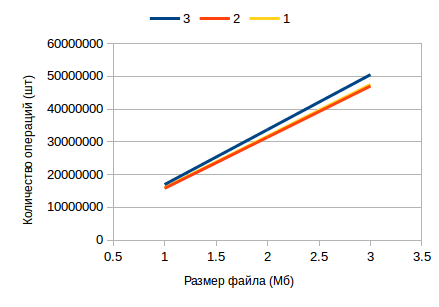
\includegraphics[width=0.5\textwidth]{graphs/1/hc_mb}
    \end{figure}
    \begin{figure}[!htb]
        \caption{Алгоритм Хаффмана, деархивирование малых файлов}
        \centering
        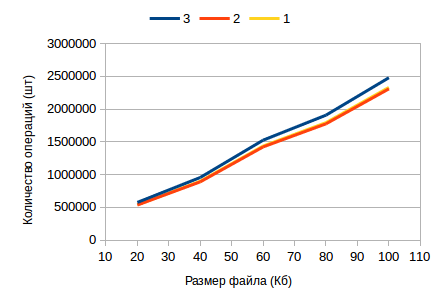
\includegraphics[width=0.5\textwidth]{graphs/1/hd_kb}
    \end{figure}
    \begin{figure}[!htb]
        \caption{Алгоритм Хаффмана, деархивирование больших файлов}
        \centering
        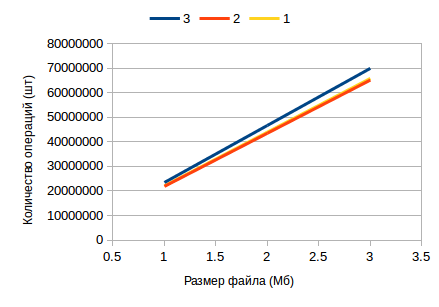
\includegraphics[width=0.5\textwidth]{graphs/1/hd_mb}
    \end{figure}
    \begin{figure}[!htb]
        \caption{Алгоритм Шеннона-Фано, архивирование малых файлов}
        \centering
        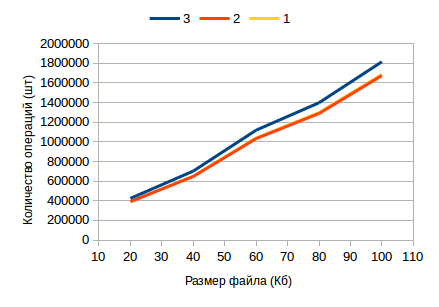
\includegraphics[width=0.5\textwidth]{graphs/1/sc_kb}
    \end{figure}
    \begin{figure}[!htb]
        \caption{Алгоритм Шеннона-Фано, архивирование больших файлов}
        \centering
        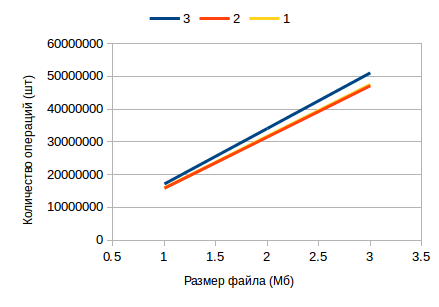
\includegraphics[width=0.5\textwidth]{graphs/1/sc_mb}
    \end{figure}
    \begin{figure}[!htb]
        \caption{Алгоритм Шеннона-Фано, деархивирование малых файлов}
        \centering
        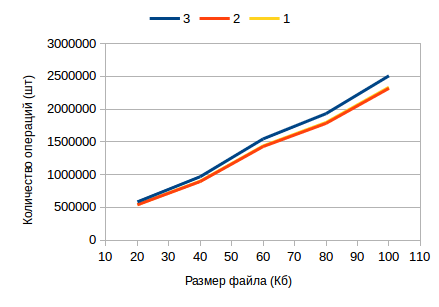
\includegraphics[width=0.5\textwidth]{graphs/1/sd_kb}
    \end{figure}
    \begin{figure}[!htb]
        \caption{Алгоритм Шеннона-Фано, деархивирование больших файлов}
        \centering
        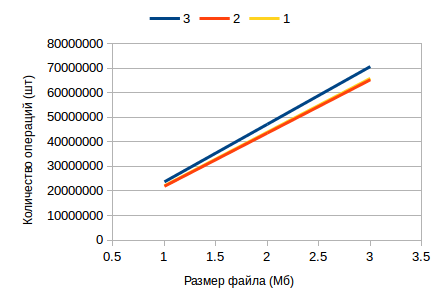
\includegraphics[width=0.5\textwidth]{graphs/1/sd_mb}
    \end{figure}
    %%%--------------------------------------------2
    \begin{figure}[!htb]
        \caption{Первый набор, архивирование малых файлов}
        \centering
        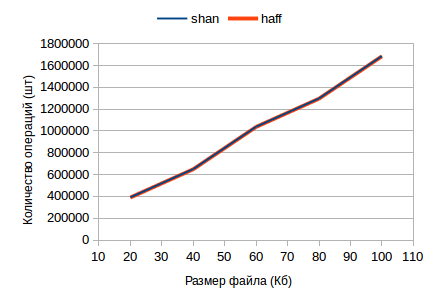
\includegraphics[width=0.5\textwidth]{graphs/2/1_c_kb}
    \end{figure}
    \begin{figure}[!htb]
        \caption{Первый набор, архивирование больших файлов}
        \centering
        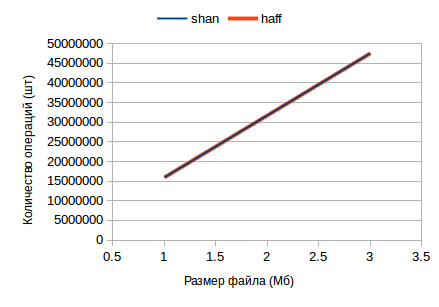
\includegraphics[width=0.5\textwidth]{graphs/2/1_c_mb}
    \end{figure}
    \begin{figure}[!htb]
        \caption{Первый набор, деархивирование малых файлов}
        \centering
        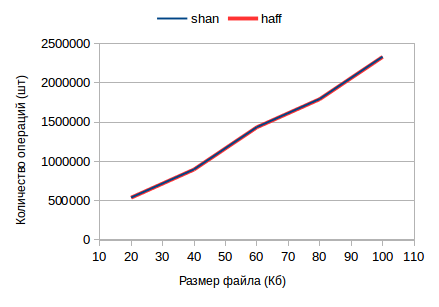
\includegraphics[width=0.5\textwidth]{graphs/2/1_d_kb}
    \end{figure}
    \begin{figure}[!htb]
        \caption{Первый набор, деархивирование больших файлов}
        \centering
        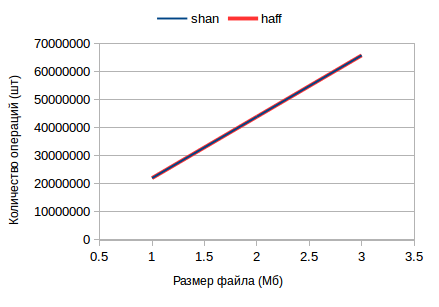
\includegraphics[width=0.5\textwidth]{graphs/2/1_d_mb}
    \end{figure}
    \begin{figure}[!htb]
        \caption{Второй набор, архивирование малых файлов}
        \centering
        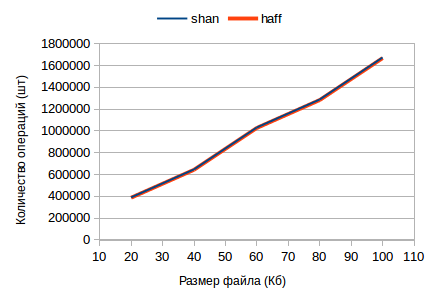
\includegraphics[width=0.5\textwidth]{graphs/2/2_c_kb}
    \end{figure}
    \begin{figure}[!htb]
        \caption{Второй набор, архивирование больших файлов}
        \centering
        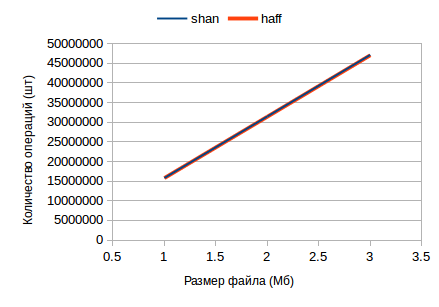
\includegraphics[width=0.5\textwidth]{graphs/2/2_c_mb}
    \end{figure}
    \begin{figure}[!htb]
        \caption{Второй набор, деархивирование малых файлов}
        \centering
        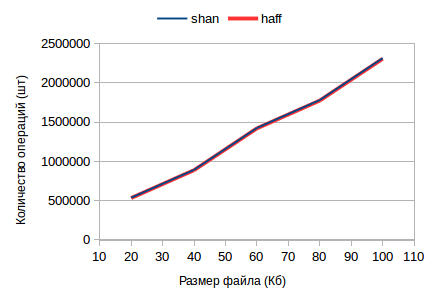
\includegraphics[width=0.5\textwidth]{graphs/2/2_d_kb}
    \end{figure}
    \begin{figure}[!htb]
        \caption{Второй набор, деархивирование больших файлов}
        \centering
        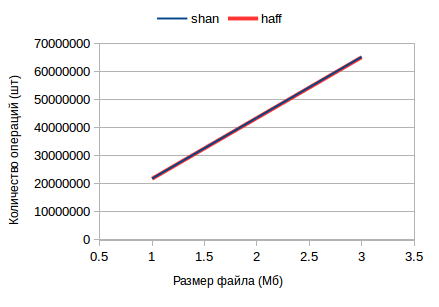
\includegraphics[width=0.5\textwidth]{graphs/2/2_d_mb}
    \end{figure}

    \begin{figure}[!htb]
        \caption{Третий набор, архивирование малых файлов}
        \centering
        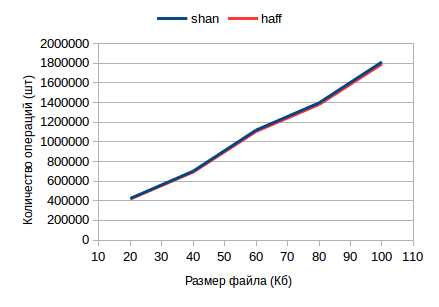
\includegraphics[width=0.5\textwidth]{graphs/2/3_c_kb}
    \end{figure}
    \begin{figure}[!htb]
        \caption{Третий набор, архивирование больших файлов}
        \centering
        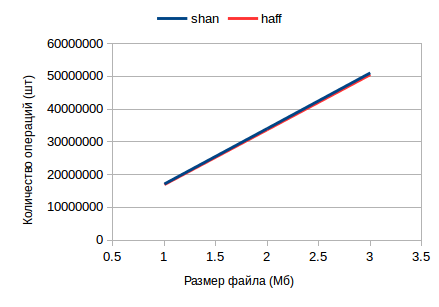
\includegraphics[width=0.5\textwidth]{graphs/2/3_c_mb}
    \end{figure}
    \begin{figure}[!htb]
        \caption{Третий набор, деархивирование малых файлов}
        \centering
        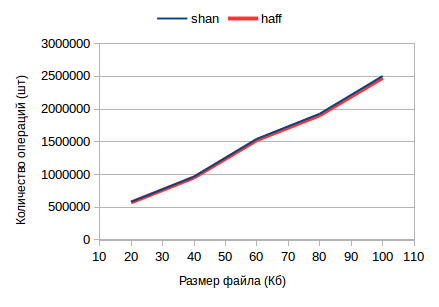
\includegraphics[width=0.5\textwidth]{graphs/2/3_d_kb}
    \end{figure}
    \begin{figure}[!htb]
        \caption{Третий набор, деархивирование больших файлов}
        \centering
        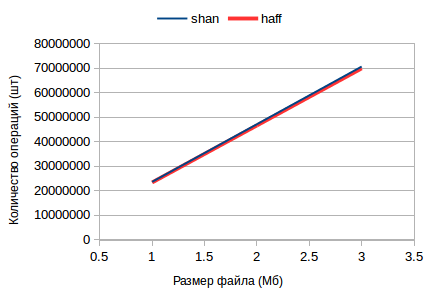
\includegraphics[width=0.5\textwidth]{graphs/2/3_d_mb}
    \end{figure}
    %%%--------------------------------------------3
    \begin{figure}[!htb]
        \caption{Файл размера 3 Мб, архивирование}
        \centering
        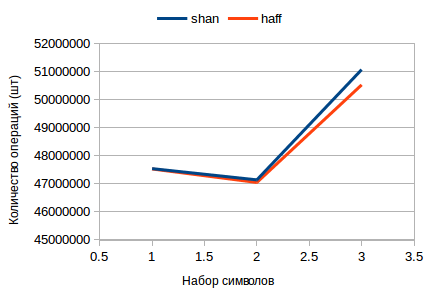
\includegraphics[width=0.5\textwidth]{graphs/3/c}
    \end{figure}
    \begin{figure}[!htb]
        \caption{Файл размера 3 Мб, деархивирование}
        \centering
        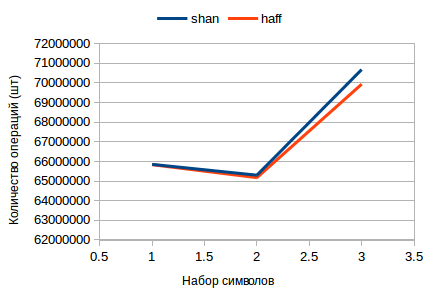
\includegraphics[width=0.5\textwidth]{graphs/3/d}
    \end{figure}
    \begin{figure}[!htb]
        \caption{Архивирование второго набора (детально)}
        \centering
        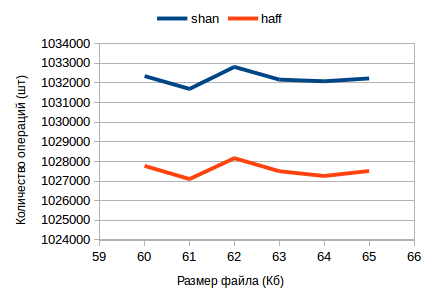
\includegraphics[width=0.5\textwidth]{graphs/2/2_c_detailed}
    \end{figure}
    \begin{figure}[!htb]
        \caption{Деархивирование второго набора (детально)}
        \centering
        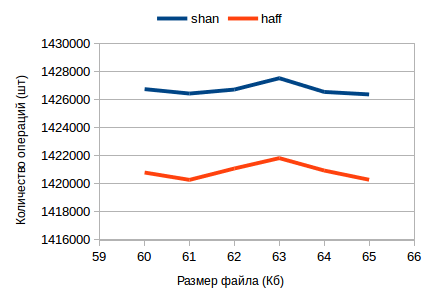
\includegraphics[width=0.5\textwidth]{graphs/2/2_d_detailed}
    \end{figure}
    %----------------------------------------------TABLES
    \begin{table}[!htb]
        \centering
        \caption{Архивирование второго набора алгоритмом Шеннона-Фано}
        \begin{tabular}{|l|l|l|l|l|}
            \hline
            algo & size & set & op\_avg \\ \hline
            shan & 100 & 2 & 1673822 \\ \hline
            shan & 80 & 2 & 1288363  \\ \hline
            shan & 60 & 2 & 1032024  \\ \hline
            shan & 40 & 2 & 647033  \\ \hline
            shan & 20 & 2 & 390287  \\ \hline
            shan & 3 & 2 & 47142032  \\ \hline
            shan & 2 & 2 & 31468055 \\ \hline
            shan & 1 & 2 & 15799812  \\ \hline
        \end{tabular}
    \end{table}
    \begin{table}[!htb]
        \centering
        \caption{Архивирование второго набора алгоритмом Хаффмана}
        \begin{tabular}{|l|l|l|l|}
            \hline
            algo & size & set & op\_avg \\ \hline
            haff & 100 & 2 & 1667656 \\ \hline
            haff & 80 & 2 & 1283284 \\ \hline
            haff & 60 & 2 & 1027498 \\ \hline
            haff & 40 & 2 & 643309 \\ \hline
            haff & 20 & 2 & 387222 \\ \hline
            haff & 3 & 2 & 47050050 \\ \hline
            haff & 2 & 2 & 31403965 \\ \hline
            haff & 1 & 2 & 15765169 \\ \hline
        \end{tabular}
    \end{table}
    \begin{table}[!htb]
        \centering
        \caption{Деархивирование второго набора алгоритмом Шеннона-Фано}
        \begin{tabular}{|l|l|l|l|}
            \hline
            algo & size & set & op\_avg \\ \hline
            shan & 100 & 2 & 2315620 \\ \hline
            shan & 80 & 2 & 1781680 \\ \hline
            shan & 60 & 2 & 1426589 \\ \hline
            shan & 40 & 2 & 893291 \\ \hline
            shan & 20 & 2 & 537642 \\ \hline
            shan & 3 & 2 & 65298550 \\ \hline
            shan & 2 & 2 & 43586900 \\ \hline
            shan & 1 & 2 & 21883098 \\ \hline
        \end{tabular}
    \end{table}
    \begin{table}[!htb]
       \centering
       \caption{Деархивирование второго набора алгоритмом Хаффмана}
        \begin{tabular}{|l|l|l|l|}
            \hline
            algo & size & set & op\_avg \\ \hline
            haff & 100 & 2 & 2307712 \\ \hline
            haff & 80 & 2 & 1775259 \\ \hline
            haff & 60 & 2 & 1420925 \\ \hline
            haff & 40 & 2 & 888725 \\ \hline
            haff & 20 & 2 & 533976 \\ \hline
            haff & 3 & 2 & 65173208 \\ \hline
            haff & 2 & 2 & 43499727 \\ \hline
            haff & 1 & 2 & 21836220 \\ \hline
        \end{tabular}
    \end{table}
    \begin{table}[!htb]
        \centering
        \caption{Алгоритм Хаффмана, архивирование разных наборов}
        \begin{tabular}{|l|l|l|}
            \hline
            size & set & op\_avg \\ \hline
            20   & 3   & 417007  \\ \hline
            40   & 3   & 692008  \\ \hline
            60   & 3   & 1104518 \\ \hline
            80   & 3   & 1380453 \\ \hline
            100  & 3   & 1793882 \\ \hline
            20   & 2   & 387142  \\ \hline
            40   & 2   & 643017  \\ \hline
            60   & 2   & 1028560 \\ \hline
            80   & 2   & 1283607 \\ \hline
            100  & 2   & 1669145 \\ \hline
            20   & 1   & 389625  \\ \hline
            40   & 1   & 648565  \\ \hline
            60   & 1   & 1036965 \\ \hline
            80   & 1   & 1295730 \\ \hline
            100  & 1   & 1684255 \\ \hline
        \end{tabular}
    \end{table}
    \begin{table}[!htb]
        \centering
        \caption{Алгоритм Хаффмана, деархивирование разных наборов}
        \begin{tabular}{|l|l|l|}
            \hline
            size & set & op\_avg \\ \hline
            20 & 3 & 574102 \\ \hline
            40 & 3 & 954732 \\ \hline
            60 & 3 & 1525688 \\ \hline
            80 & 3 & 1907595 \\ \hline
            100 & 3 & 2479808 \\ \hline
            20 & 2 & 533868 \\ \hline
            40 & 2 & 888324 \\ \hline
            60 & 2 & 1422378 \\ \hline
            80 & 2 & 1775701 \\ \hline
            100 & 2 & 2309748 \\ \hline
            20 & 1 & 538571 \\ \hline
            40 & 1 & 897222 \\ \hline
            60 & 1 & 1435184 \\ \hline
            80 & 1 & 1793597 \\ \hline
            100 & 1 & 2331731 \\ \hline
        \end{tabular}
    \end{table}
    \clearpage
    \section{Сравнительный анализ методов}
    \subsection{Количество операций}
    \begin{itemize}
        \item
        Поскольку на некоторых графиках (Рис. 9 --- Рис. 20) два алгоритма архивирования/деархивирования показывают 
        практически одинаковые результаты, в Таблице 1 --- Таблице 4 приведены конкретные значения, а на Рис. 23 и Рис. 24
        представлены более детальные графики. Таким образом, можно заметить, что алгоритм Хаффмана работает быстрее (а 
        именно за меньшее число операций строится кодовое дерево), чем алгоритм Шеннона-Фано, пусть и незначительно. 
        \item
        Что касается наборов файлов размера 3 Мб, то здесь алгоритм Хаффмана однозначно работает быстрее на третьем 
        наборе.
        Но неожиданно, что, хотя 1-й набор содержит меньше различных символов, архивируется/деархивируется он чуть 
        медленнее, чем 2-й набор. Это видно на Рис. 21 и Рис. 22. 
        \item
        Также на Рис. 1 --- Рис. 8 видно, что файлы из 3-го набора архивируются/деархивируются медленнее, так как
        содержат значительно больше различных символов (знаки пунктуации и т.д.). Файлы из 1-го и 2-го набора при этом 
        архивируются/деархивируются примерно за одинаковое  количество операций (Таблица 5, Таблица 6). 
    \end{itemize}
    \subsection{Степень сжатия}
    $$\text{Степень сжатия}=\frac{\text{Размер выходного файла}}{\text{Размер входного файла}}$$
    \begin{itemize}
        \item
        Степень сжатия алгоритмом Хаффмана = 0.7477680191
        \item
        Степень сжатия алгоритмом Шеннона-Фано = 0.752124972
    \end{itemize}
    Разумеется, для файлов низким размером степень сжатия будет больше единицы, так как
    в начало архивированного файла записывается дополнительная информация. Например, файл размера 9 байт после
    сжатия алгоритмом Хаффмана имеет размер 56 байт.\\
    Тестовый набор содержит случайно сгенерированные файлы, поэтому частота встречаемости каждого символа может
    быть примерно одинаковой. Для наглядности был сжат первый том произведения "Война и мир":
    \newpage
    \begin{itemize}
        \item
        Исходный размер = 2.6 Мб
        \item
        Размер сжатого файла алгоритмом Хаффмана = 1.3 Мб
        \item
        Размер сжатого файла алгоритмом Шеннона-Фано = 1.4 Мб
    \end{itemize}
    Таким образом, степень сжатия уже приблизительно равна 0.5, что намного лучше, чем при архивации 
    случайно сгенерированных файлов.
    \newpage
    \section{Выводы}
    \begin{itemize}
        \item
        Степень сжатия у алгоритма Хаффмана немного лучше, чем у алгоритма
        Шеннона-Фано.
        \item
        Алгоритм Хаффмана работает слегка быстрее, чем алгоритм Шеннона-Фано.
        \item
        Файлы с более разнообразным набором символов архивируются/деархивируются
        дольше.
        \item
        Файлы с реальным текстом сжимаются лучше случайно сгенерированных. Это происходит потому, что
        используются ограниченный набор символов, слова повторяются и в принципе прослеживается некоторая
        закономерность в построении предложений и текста.
    \end{itemize}
    В целом резльтат эксперимента оказался достаточно предсказуемым: алгоритм Хаффмана показывает лучшие
    результаты, чем алгоритм Шеннона-Фано. Собственно, это и требовалось проверить.

    \newpage
    \section{Использованные источники}
    \begin{enumerate}
        \item
        Новиков Ф. А. Дискретная математика для программистов: Учебник для вузов. 3-е изд. —
        СПб.: Питер, 2009. ISBN 978-5-91180-759-7
        \item
        Кормен, Томас X., Лейзерсон, Чарльз И., Ривест, Рональд Л., Штайн, Клиффорд. Алгоритмы: построение
        и анализ, 2-е издание. : Пер. с англ. М.: Издательский дом "Вильямc", 2005. ISBN 5-8459-0857-4
    \end{enumerate}
\end{document} % конец документа